\documentclass[tikz,border=5pt]{standalone}
\usepackage[utf8]{inputenc}
\usepackage[T1]{fontenc}
\usepackage{lmodern,amsmath,amssymb}
\usepackage[american]{circuitikz}
\usepackage{pgfplots}
\pgfplotsset{compat=1.18}
\usetikzlibrary{circuits.logic.US,positioning,calc,arrows.meta,patterns,shapes.geometric}
\definecolor{Primary}{HTML}{1F77B4}
\begin{document}
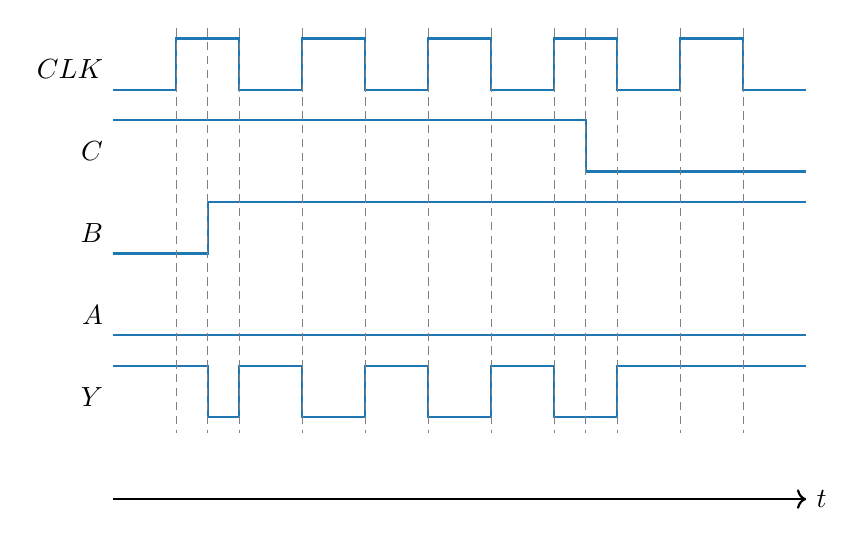
\begin{tikzpicture}[x=.8cm,y=.65cm,thick]\node[left]at(0,0.4){$ CLK $};\draw[Primary] (0,0.0)--(1,0.0)--(1,1.0)--(2,1.0)--(2,0.0)--(3,0.0)--(3,1.0)--(4,1.0)--(4,0.0)--(5,0.0)--(5,1.0)--(6,1.0)--(6,0.0)--(7,0.0)--(7,1.0)--(8,1.0)--(8,0.0)--(9,0.0)--(9,1.0)--(10,1.0)--(10,0.0)--(11,0.0);\node[left]at(0,-1.2000000000000002){$ C $};\draw[Primary] (0,-0.6000000000000001)--(7.5,-0.6000000000000001)--(7.5,-1.6)--(11,-1.6);\node[left]at(0,-2.8000000000000003){$ B $};\draw[Primary] (0,-3.2)--(1.5,-3.2)--(1.5,-2.2)--(11,-2.2);\node[left]at(0,-4.4){$ A $};\draw[Primary] (0,-4.800000000000001)--(11,-4.800000000000001);\node[left]at(0,-6.0){$ Y $};\draw[Primary] (0,-5.4)--(1.5,-5.4)--(1.5,-6.4)--(2,-6.4)--(2,-5.4)--(3,-5.4)--(3,-6.4)--(4,-6.4)--(4,-5.4)--(5,-5.4)--(5,-6.4)--(6,-6.4)--(6,-5.4)--(7,-5.4)--(7,-6.4)--(8,-6.4)--(8,-5.4)--(11,-5.4);\draw[gray,densely dashed,thin](1,1.2)--(1,-6.7);\draw[gray,densely dashed,thin](1.5,1.2)--(1.5,-6.7);\draw[gray,densely dashed,thin](2,1.2)--(2,-6.7);\draw[gray,densely dashed,thin](3,1.2)--(3,-6.7);\draw[gray,densely dashed,thin](4,1.2)--(4,-6.7);\draw[gray,densely dashed,thin](5,1.2)--(5,-6.7);\draw[gray,densely dashed,thin](6,1.2)--(6,-6.7);\draw[gray,densely dashed,thin](7,1.2)--(7,-6.7);\draw[gray,densely dashed,thin](7.5,1.2)--(7.5,-6.7);\draw[gray,densely dashed,thin](8,1.2)--(8,-6.7);\draw[gray,densely dashed,thin](9,1.2)--(9,-6.7);\draw[gray,densely dashed,thin](10,1.2)--(10,-6.7);\draw[->](0,-8.0)--(11,-8.0)node[right]{$t$};\end{tikzpicture}
\end{document}
